\section*{Machine Learning Algorithms}
\addcontentsline{toc}{section}{Machine Learning Algorithms}
\fancyhead[R]{Machine Learning Algorithms}

\section*{Supervised Machine Learning}
Supervised Machine Learning is the task of learning a function which maps an input to an output based on example input-output pairs. A supervised Machine learning algorithm analyzes the training data and produces an inferred function, which can be used for mapping new examples. An optimal scenario will allow for the algorithm to correctly determine the class labels or predict the values for unseen instances.\\
It is further divided into 2 types:
\begin{description}
    \item[Classification:]{takes real value input and produces a discrete output}
    \item[Regression]{takes real value as input and produces a continuous output}
\end{description}


\subsection*{Linear Regression}
\addcontentsline{toc}{subsection}{Linear Regression}
\begin{figure}[!ht]
	\centering
	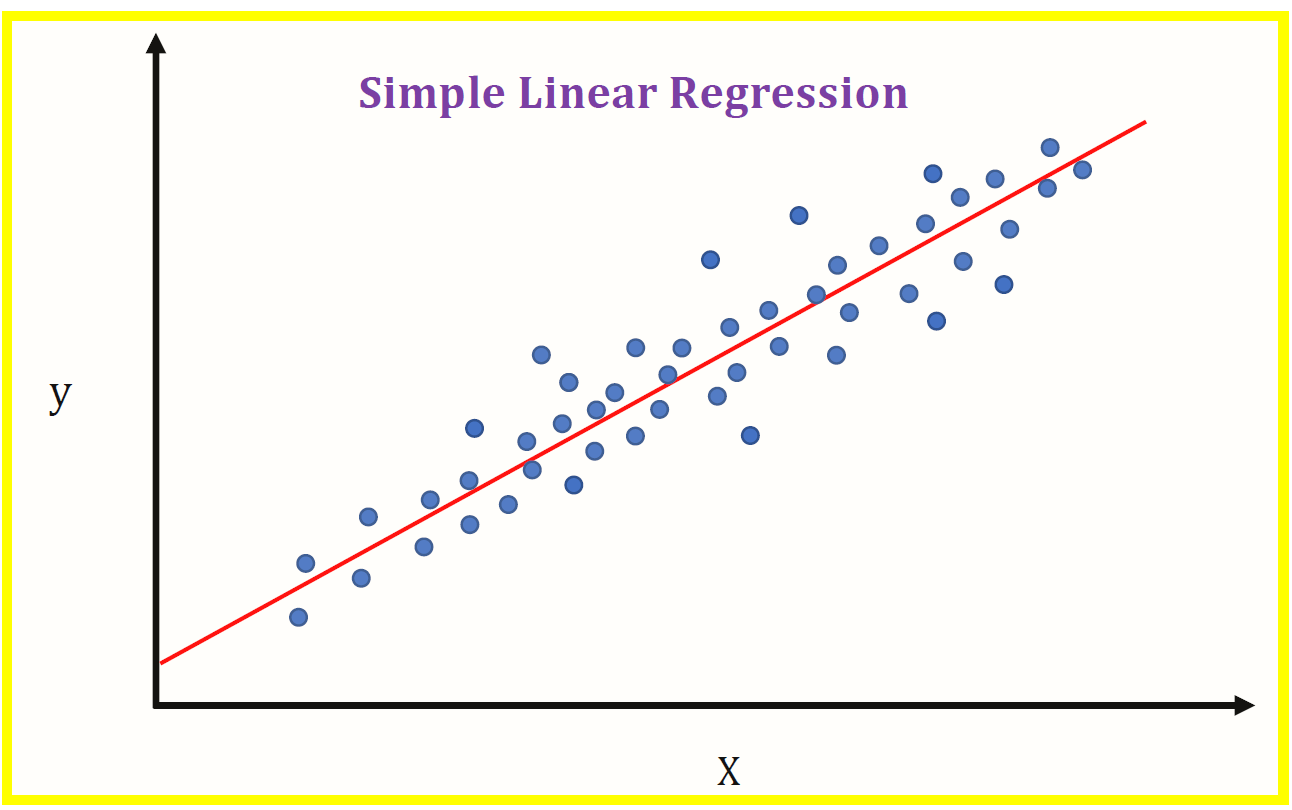
\includegraphics[width=0.8\textwidth]{images/linear-regression.png}
	\caption{Simple Linear Regression}
	\centering
	\label{label:file_name}
\end{figure}
In statistics, linear regression is a linear approach to modelling the relationship between a scalar response and one or more explanatory variables (also known as dependent and independent variables). The case of one explanatory variable is called simple linear regression; for more than one, the process is called multiple linear regression.\\
\\
Linear Regression is the first type of regression algorithm to be studied rigorously, and to be used extensively in practical applications as the models which depend linearly on their unknown parameters are easier to fit than models which are non-linearly related to their parameters.


\subsection*{Logistic Regression}
\addcontentsline{toc}{subsection}{Logistic Regression}
\begin{figure}[!ht]
	\centering
	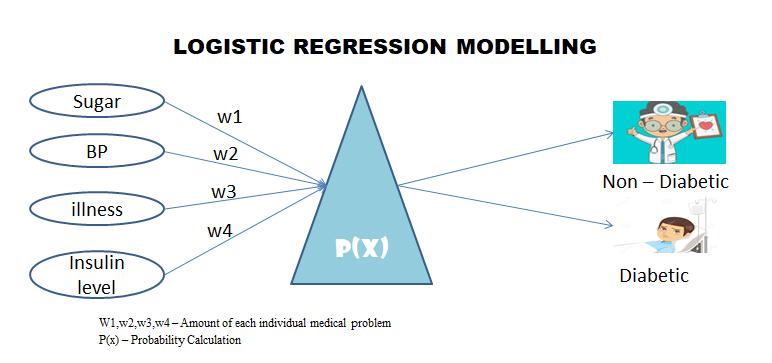
\includegraphics[width=0.8\textwidth]{images/logistic-regression.png}
	\caption{Logistic Regression Modelling}
	\centering
	\label{label:logistic}
\end{figure}
In statistics, the logistic model is used to model the probability of a certain class or event existing such as pass/fail, win/lose, alive/dead or healthy/sick. This can be extended to model several classes of events such as determining whether an image contains a cat, dog, lion, etc. Each object being detected in the image would be assigned a probability between 0 and 1, with a sum of one.\\
\\
It is named after the logistic function, also called the sigmoid function was developed by statisticians to describe properties of population growth in ecology, rising quickly and maxing out at the carrying capacity of the environment. It’s an S-shaped curve that can take any real-valued number and map it into a value between 0 and 1, but never exactly at those limits.


\subsection*{Decision Tree}
\addcontentsline{toc}{subsection}{Decision Tree}
\begin{figure}[!ht]
	\centering
	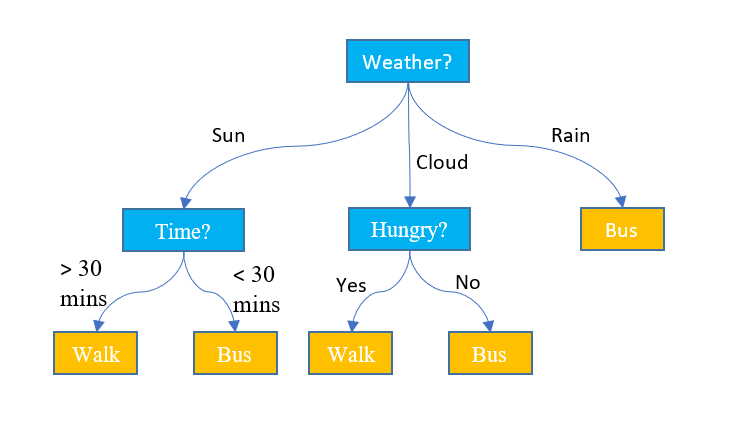
\includegraphics[width=0.8\textwidth]{images/decision-tree.png}
	\caption{Decision Tree example}
	\centering
	\label{label:decision-tree}
\end{figure}
In decision analysis, a decision tree can be used to visually and explicitly represent decisions and decision making. As the name goes, it uses a tree-like model of decisions. Though a commonly used tool in data mining for deriving a strategy to reach a particular goal, its also widely used in machine learning.\\
\\
Decision trees classify instances by sorting them down the tree from the root to some leaf node, which provides the classification of the instance. An instance is classified by starting at the root node of the tree, testing the attribute specified by this node, then moving down the tree branch corresponding to the value of the attribute. This process is then repeated for the subtree rooted at the new node.\\
Some Strengths of Decision tree approach are:
\begin{itemize}
    \item they are able to generate understandable rules.
    \item perform classification without requiring much computation.
    \item they are able to handle both continuous and categorical variables.
    \item they provide a clear indication of which fields are most important for prediction or classification.
\end{itemize}

Some of its weaknesses include:
\begin{itemize}
    \item they are less appropriate for estimation tasks where the goal is to predict the value of a continuous attribute.
    \item they are prone to errors in classification problems with many class and relatively small number of training examples.
    \item they can be computationally expensive to train.
\end{itemize}


\subsection*{Random Forest}
\addcontentsline{toc}{subsection}{Random Forest}
\begin{figure}[!ht]
	\centering
	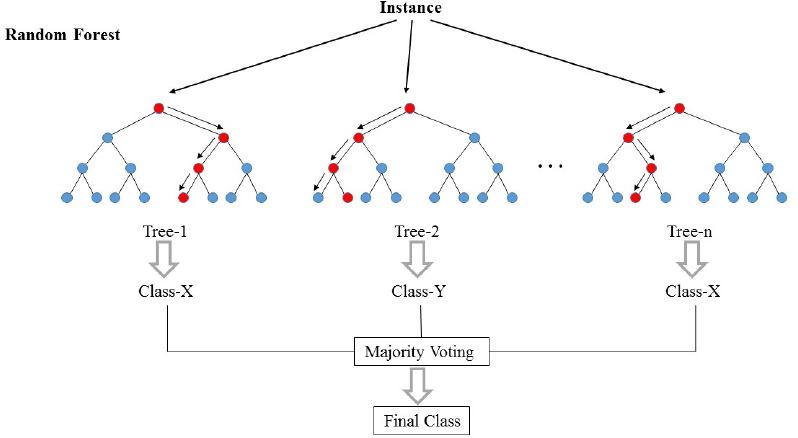
\includegraphics[width=0.8\textwidth]{images/random-forest.jpg}
	\caption{Random Forest Classification}
	\centering
	\label{label:randomforest}
\end{figure}
Random forests or random decision forests are an ensemble learning method for classification, regression and other tasks that operates by constructing a multitude of decision trees at training time.For classification tasks, the output of the random forest is the class selected by most trees. For regression tasks, the mean or average prediction of the individual trees is returned.\\
\\
Random decision forests correct for decision trees habit of overfitting to their training set. They generally outperform decision trees, however data characteristics can affect their performance. It adds additional randomness to the model, while growing the trees. Instead of searching for the most important feature while splitting a node, it searches for the best feature among a random subset of features. This results in a wide diversity that generally results in a better model.\\
\\
Random forests are frequently used as "blackbox" models in businesses, as they generate reasonable predictions across a wide range of data while requiring little configuration.

\subsection*{Bayes Classifier}
\addcontentsline{toc}{subsection}{Bayes Classifier}
In statistics, naive Bayes classifiers are a family of simple "probabilistic classifiers" based on applying Bayes' theorem with strong independence assumptions between the features. They are among the simplest Bayesian network models.\\
\\
They are among the simplest Bayesian network models. Despite their naive design and apparently oversimplified assumptions, naive Bayes classifiers have worked quite well in many complex real-world situations.\\
An advantage of naive Bayes is that it only requires a small number of training data to estimate the parameters necessary for classification.


\subsection*{K{-}Nearest Neighbors(KNN)}
\addcontentsline{toc}{subsection}{K{-}Nearest Neighbors}
\begin{figure}[!ht]
	\centering
	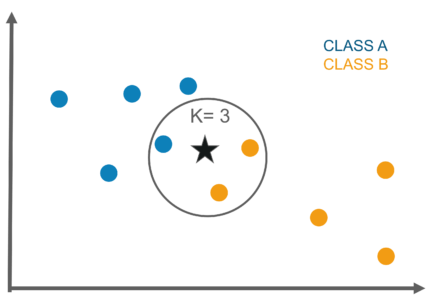
\includegraphics[width=0.8\textwidth]{images/knn.png}
	\caption{Classifying unknown example with K=3}
	\centering
	\label{label:knn}
\end{figure}
The k-nearest neighbors (KNN) algorithm is a simple, supervised machine learning algorithm that can be used to solve both classification and regression problems. It’s easy to implement and understand, but has a major drawback of becoming significantly slows as the size of that data in use grows.\\
\\
KNN works by finding the distances between a query and all the examples in the data, selecting the specified number examples (K) closest to the query, then votes for the most frequent label (in the case of classification) or averages the labels (in the case of regression).


\subsection*{Support Vector Machines(SVM)}
\addcontentsline{toc}{subsection}{Support Vector Machines}
\begin{figure}[!ht]
	\centering
	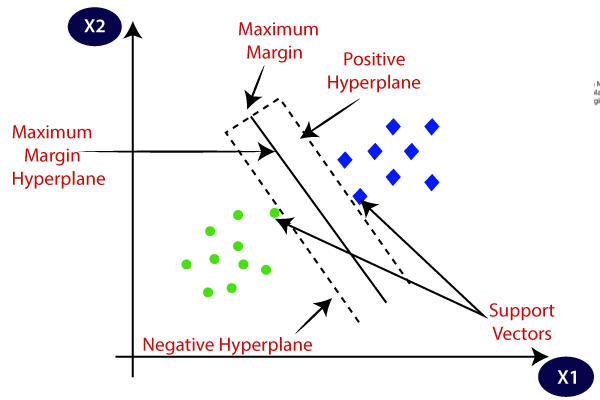
\includegraphics[width=0.8\textwidth]{images/svm.png}
	\caption{Support Vector Machine example}
	\centering
	\label{label:svm}
\end{figure}
“Support Vector Machine” (SVM) is a supervised machine learning algorithm which can be used for both classification or regression challenges. However,  it is mostly used in classification problems. In the SVM algorithm, we plot each data item as a point in n{-}dimensional space (where n is number of features you have) with the value of each feature being the value of a particular coordinate. Then, we perform classification by finding the hyper-plane that differentiates the two classes.\\
\\
Hyperplanes are decision boundaries that help classify the data points. Data points falling on either side of the hyperplane can be attributed to different classes. Also, the dimension of the hyperplane depends upon the number of features. If the number of input features has dimension n, then the hyperplane will be a (n-1) dimensional affine plane.\\
\\
Support Vectors are simply the co-ordinates of individual observation. The SVM classifier is a frontier which best segregates the two classes (hyper-plane/ line).